\section{Observation of Approximation Errors}
To study the character of approximation errors we first made a few experimental
observations on generated data.

\subsection{Data Generation}
\label{sec:data-generation}
Since we will later use the approximated histogram to estimate a genome size, 
we will mainly study Kmerlight's performance on the data that are to some
degree biologically plausible. We will base our data generation on a sequencing
process as it was described in section \ref{sec:sequencing}.

As the Kmerlight's input data consist of genome reads, we first generate a genome $g_1g_2g_3 \dots g_L$:
a random sequence of length $L$ consisting of characters $A, C, G, T$ each with probabilty $1/4$ at every position.

Aftewards we generate reads each of length $l=100$. Instead of creating an explicit number of reads, we choose
a parameter $c$ (coverage) and generate $c \cdot L / l$ independent reads.

To generate a single read we uniformly select a random starting position $s$ in genome from a range $1, \dots, L - l + 1$
and then the read consists of characters $g_s g_{s+1} \dots g_{s+l-1}$. Finally, to simulate sequencing errors,
we change each read character with probabilty $e/3$ ($e$ denotes error rate) into a one of the three other characters.

With parameters $L, c, e$ we are able to mimic the real squencing data and they provide us with suffucient freedom.

% TODO: link sources from covest github

\subsection{Error characteristics}

In this section we compare exact $k$-mer abundance histogram produced by Jellyfish software
to approximated histograms computed by Kmerlight (with parameters $t=7, r=2^{15}, u=2^{13}$ using 60MB of RAM).
We executed Kmerlight in 50 trials with the same input data and we investigate means and standard deviations of 
the estimates $\hat f_i$. We demostrate three error characteristics on a genome generated with parameters $L=10^6, c=50, e=0.02$.

\paragraph{Overestimation}
In figure \ref{img:exact-vs-approximated-histogram} it is clearly visible, that Kmerlight systematically overestimates values of $f_i$.
Mean errors for abundances around 25 reach absolute values of 4000.


\begin{figure}[h]
\centerline{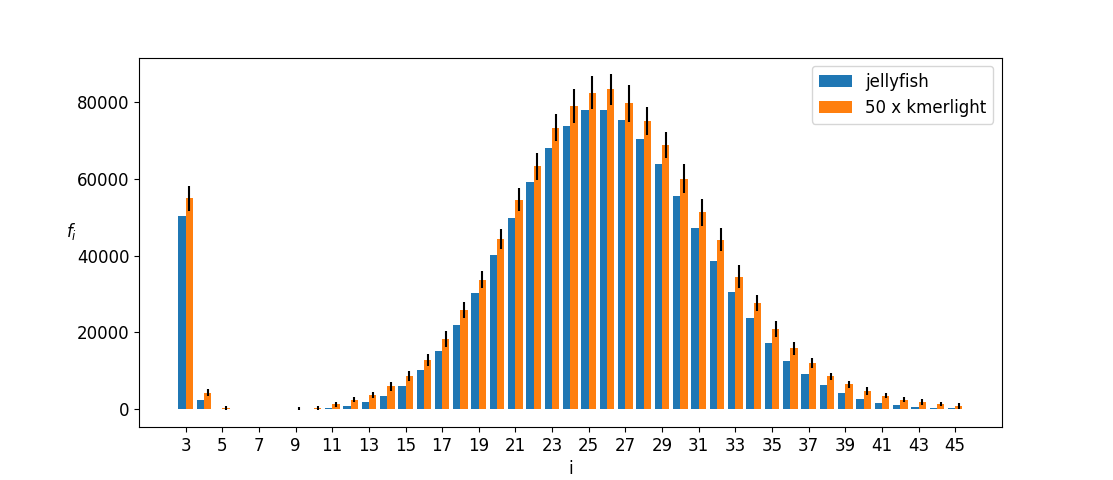
\includegraphics[width=1\textwidth, trim={1.5cm, 0cm, 2.5cm, 1.3cm}, clip]{{images/histogram_errors_L1000000_c50_e0.02_k21_normal}.png}}
\caption[Comparison of exact and approximated histograms]{Values of exact $f_i$ produced by Jellyfish software (blue)
and approximated values $\hat f_i$ produced by Kmerlight averaged from 50 trials (orange). The errorbars experss the
standard deviation of each estimate. Note that columns for $i=1,2$ were trimmed having values $10^7, 10^6$ respectively.}
\label{img:exact-vs-approximated-histogram}
\end{figure}

\begin{figure}[h]
\centerline{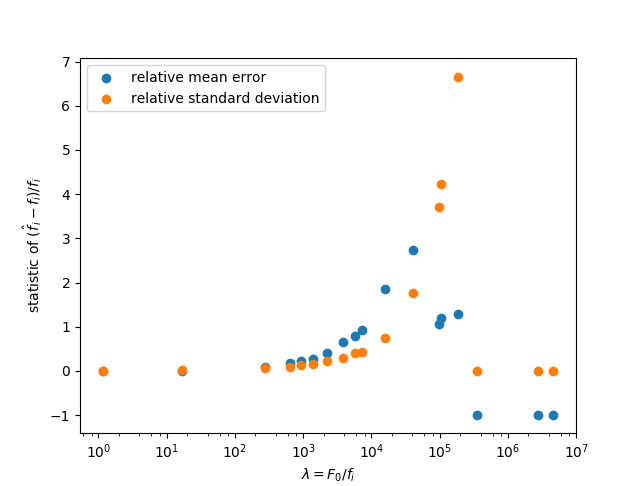
\includegraphics[width=1\textwidth, trim={0cm, 0cm, 0cm, 0cm}, clip]{{images/relative_errors_mean_std_L1000000_c50_e0.02_k21_normal}.png}}
\caption[Relative approximation errors]{}
\label{img:relative-errors}
\end{figure}

\paragraph{Insensivity to lowest $f_i$}

\begin{figure}[h]
\centerline{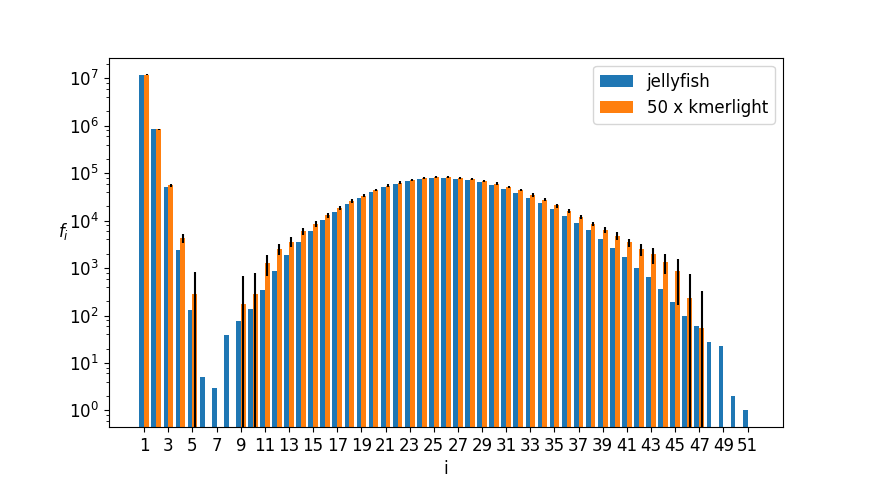
\includegraphics[width=1\textwidth, trim={2cm, 0cm, 2.5cm, 1.3cm}, clip]{{images/histogram_errors_L1000000_c50_e0.02_k21_normal_log}.png}}
\caption[Comparison of exact and approximated histograms in log scale]{}
\label{img:exact-vs-approximated-histogram-log}
\end{figure}
